\begin{figure}[h!]
	\centering
	
	
	
	\tikzset{every picture/.style={line width=0.75pt}} %set default line width to 0.75pt        
	
	\begin{tikzpicture}[x=0.75pt,y=0.75pt,yscale=-1,xscale=1]
		%uncomment if require: \path (0,300); %set diagram left start at 0, and has height of 300
		
		%Straight Lines [id:da13324820830621897] 
		\draw    (182,70) -- (250,70) ;
		\draw [shift={(180,70)}, rotate = 0] [color={rgb, 255:red, 0; green, 0; blue, 0 }  ][line width=0.75]    (10.93,-3.29) .. controls (6.95,-1.4) and (3.31,-0.3) .. (0,0) .. controls (3.31,0.3) and (6.95,1.4) .. (10.93,3.29)   ;
		%Straight Lines [id:da5531596119865458] 
		\draw    (182,150) -- (250,150) ;
		\draw [shift={(180,150)}, rotate = 0] [color={rgb, 255:red, 0; green, 0; blue, 0 }  ][line width=0.75]    (10.93,-3.29) .. controls (6.95,-1.4) and (3.31,-0.3) .. (0,0) .. controls (3.31,0.3) and (6.95,1.4) .. (10.93,3.29)   ;
		%Straight Lines [id:da6403367281349892] 
		\draw    (160,80) -- (159.85,86.57) -- (159.04,122.6) ;
		\draw [shift={(159,124.6)}, rotate = 271.28] [color={rgb, 255:red, 0; green, 0; blue, 0 }  ][line width=0.75]    (10.93,-3.29) .. controls (6.95,-1.4) and (3.31,-0.3) .. (0,0) .. controls (3.31,0.3) and (6.95,1.4) .. (10.93,3.29)   ;
		%Straight Lines [id:da1275719919912266] 
		\draw    (270,80) -- (269.04,122.6) ;
		\draw [shift={(269,124.6)}, rotate = 271.28] [color={rgb, 255:red, 0; green, 0; blue, 0 }  ][line width=0.75]    (10.93,-3.29) .. controls (6.95,-1.4) and (3.31,-0.3) .. (0,0) .. controls (3.31,0.3) and (6.95,1.4) .. (10.93,3.29)   ;
		%Straight Lines [id:da19337619875864354] 
		\draw    (260,80) -- (181.7,128.94) ;
		\draw [shift={(180,130)}, rotate = 327.99] [color={rgb, 255:red, 0; green, 0; blue, 0 }  ][line width=0.75]    (10.93,-3.29) .. controls (6.95,-1.4) and (3.31,-0.3) .. (0,0) .. controls (3.31,0.3) and (6.95,1.4) .. (10.93,3.29)   ;
		
		% Text Node
		\draw (153,52.4) node [anchor=north west][inner sep=0.75pt]    {$H{^{2}}$};
		% Text Node
		\draw (259,59.4) node [anchor=north west][inner sep=0.75pt]    {$S^{2}$};
		% Text Node
		\draw (146,126.4) node [anchor=north west][inner sep=0.75pt]    {$\dfrac{H^{2}}{\sim }$};
		% Text Node
		\draw (256,126.4) node [anchor=north west][inner sep=0.75pt]    {$\dfrac{S^{2}}{\sim }$};
		% Text Node
		\draw (197.27,101.99) node [anchor=north west][inner sep=0.75pt]  [font=\scriptsize,rotate=-327.41]  {$\pi _{1} \circ k$};
		% Text Node
		\draw (141,92.4) node [anchor=north west][inner sep=0.75pt]  [font=\scriptsize]  {$\pi _{1}$};
		% Text Node
		\draw (274,96.4) node [anchor=north west][inner sep=0.75pt]  [font=\scriptsize]  {$\pi _{2}$};
		% Text Node
		\draw (208,152.4) node [anchor=north west][inner sep=0.75pt]  [font=\scriptsize]  {$g$};
		% Text Node
		\draw (210,54.4) node [anchor=north west][inner sep=0.75pt]  [font=\scriptsize]  {$k$};
		
		
	\end{tikzpicture}
\end{figure}